\begin{figure}[t]
\centering
    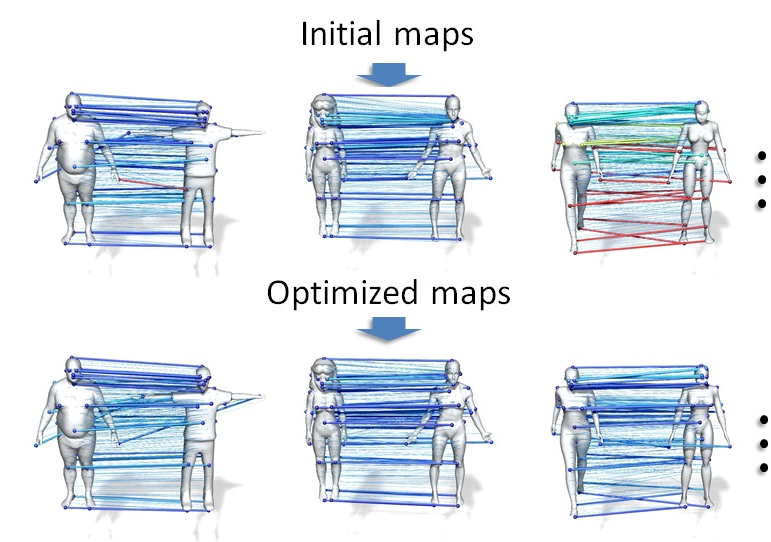
\includegraphics[width=1.0\columnwidth]{fig/img/huang_sig14_jsm.png}
    %\vspace{-0.4cm}
    \caption{Joint shape matching takes as input maps computed between pairs of shapes in isolation and utilizes the cycle-consistency constraint to improve shape maps. This figure shows the result of Huang et al.~\protect\cite{Huang:2014:FMN}, which performs joint shape matching under the functional map setting.}
    \label{fig:huang_sig14_jsm}
\end{figure}

